\section{方法设计与转换测试单元}
本章集中放置符号表、图片、算法和自定义编号列表。所有元素都在正文中进行交叉引用，便于检查Word中引用文字是否显示为“表x-y”“图x-y”“算法x-y”和“式x-y”。

\subsection{问题定义与符号说明}
给定一个包含MoE层的视觉语言模型$\mathcal{M}$，专家压缩的目标是在保留任务性能的前提下降低每层专家数量。设压缩保留比例为$r=M/N$，压缩过程可表述为\eqnref{eq:compression_objective}。
\begin{equation}
    \label{eq:compression_objective}
    \mathcal{M}' = \arg\min_{\mathcal{M}'} \; \mathbb{E}_{x \sim \mathcal{D}} \left[ \mathcal{L}(\mathcal{M}', x) \right], \quad \text{s.t.} \; |\mathcal{E}_l'| = M, \; \forall l \in \{1, \dots, L\}
\end{equation}

为便于后续描述，\tabref{chart:symbols}列出了本章使用的主要符号及其含义。该表用于检查两列表格中数学符号、中文说明和列宽自适应效果。

\begin{table}[!ht]
    \centering
    \caption{主要符号说明}
    \label{chart:symbols}
    \begin{tabular}{cl}
    \toprule
        符号 & 含义 \\ \midrule
        $\mathcal{M}$ & 原始MoE视觉语言模型 \\
        $\mathcal{M}'$ & 压缩后的模型 \\
        $L$ & MoE层总数 \\
        $N$ & 每层原始专家数量 \\
        $M$ & 每层压缩后保留的专家数量 \\
        $r$ & 压缩保留比例，$r=M/N$ \\
        $B^{(l,e)}$ & 第$l$层第$e$个专家的桥接分数 \\
        $A^{(l,e)}$ & 第$l$层第$e$个专家的模态亲和度 \\
    \bottomrule
    \end{tabular}
\end{table}

\subsection{桥接分数计算流程}
桥接分数用于估计专家对图文对应关系的敏感程度。参考DeepSeek-VL2等MoE视觉语言模型的输入组织方式\cite{wu2024deepseekvl2}，测试样例将一次校准样本拆分为四路前向输入：

\begin{list}{（\arabic{enumi}）}{
  \setlength{\leftmargin}{0pt}
  \settowidth{\labelwidth}{（1）}
  \setlength{\labelsep}{0pt}
  \setlength{\itemindent}{\dimexpr\parindent+\labelwidth\relax}
  \setlength{\itemsep}{\parskip}
  \setlength{\parsep}{0pt}
  \setlength{\topsep}{0pt}
  \setlength{\partopsep}{0pt}
  \usecounter{enumi}
}
\setlength{\parindent}{\originalparindent}
    \item 原始输入$x$：同时包含匹配的图像和文本信息；
    \item 图像扰动输入$\tilde{x}_{\mathrm{vis}}$：替换图像，文本保持不变；
    \item 文本扰动输入$\tilde{x}_{\mathrm{txt}}$：替换问题文本，图像保持不变；
    \item 图文错配输入$\tilde{x}_{\mathrm{mis}}$：保留问题文本，但替换为另一张图像。
\end{list}

\subsection{多级文字列表测试}
论文正文允许出现文字列表，但列表编号应遵循固定层级。以下三组 list 环境用于检查 DOCX 转换后是否分别显示为一级编号、二级编号和三级编号。

一级编号使用中文括号数字：
\begin{list}{（\arabic{enumi}）}{
  \setlength{\leftmargin}{0pt}
  \settowidth{\labelwidth}{（1）}
  \setlength{\labelsep}{0pt}
  \setlength{\itemindent}{\dimexpr\parindent+\labelwidth\relax}
  \setlength{\itemsep}{\parskip}
  \setlength{\parsep}{0pt}
  \setlength{\topsep}{0pt}
  \setlength{\partopsep}{0pt}
  \usecounter{enumi}
}
\setlength{\parindent}{\originalparindent}
    \item 一级列表第一项：用于检查编号是否显示为（1），且正文能够正常换行。
    \item 一级列表第二项：用于检查同一列表内编号是否连续递增。
    \item 一级列表第三项：用于检查列表结束后后续段落是否恢复普通正文格式。
\end{list}

二级编号使用带圈数字：
\begin{list}{\circlednumber{\value{enumii}}}{
  \setlength{\leftmargin}{0pt}
  \settowidth{\labelwidth}{\circlednumber{1}}
  \setlength{\labelsep}{0pt}
  \setlength{\itemindent}{\dimexpr\parindent+\labelwidth\relax}
  \setlength{\itemsep}{\parskip}
  \setlength{\parsep}{0pt}
  \setlength{\topsep}{0pt}
  \setlength{\partopsep}{0pt}
  \usecounter{enumii}
}
\setlength{\parindent}{\originalparindent}
    \item 二级列表第一项：用于检查编号是否显示为\circlednumber{1}。
    \item 二级列表第二项：用于检查带圈数字是否与中文正文保持同一行。
\end{list}

三级编号使用大写英文字母：
\begin{list}{\Alph{enumiii}}{
  \setlength{\leftmargin}{0pt}
  \settowidth{\labelwidth}{A}
  \setlength{\labelsep}{0pt}
  \setlength{\itemindent}{\dimexpr\parindent+\labelwidth\relax}
  \setlength{\itemsep}{\parskip}
  \setlength{\parsep}{0pt}
  \setlength{\topsep}{0pt}
  \setlength{\partopsep}{0pt}
  \usecounter{enumiii}
}
\setlength{\parindent}{\originalparindent}
    \item 三级列表A项：用于检查编号是否显示为A。
    \item 三级列表B项：用于检查英文字母编号是否继续递增。
    \item 三级列表C项：用于检查多级列表测试覆盖到第三层。
\end{list}

\figref{fig:merge_constraint_flow}展示了专家合并约束的流程图。该图片来自源论文图件，用于检查PNG图片尺寸、居中、图题编号和正文引用。

\begin{figure}[!ht]
    \centering
    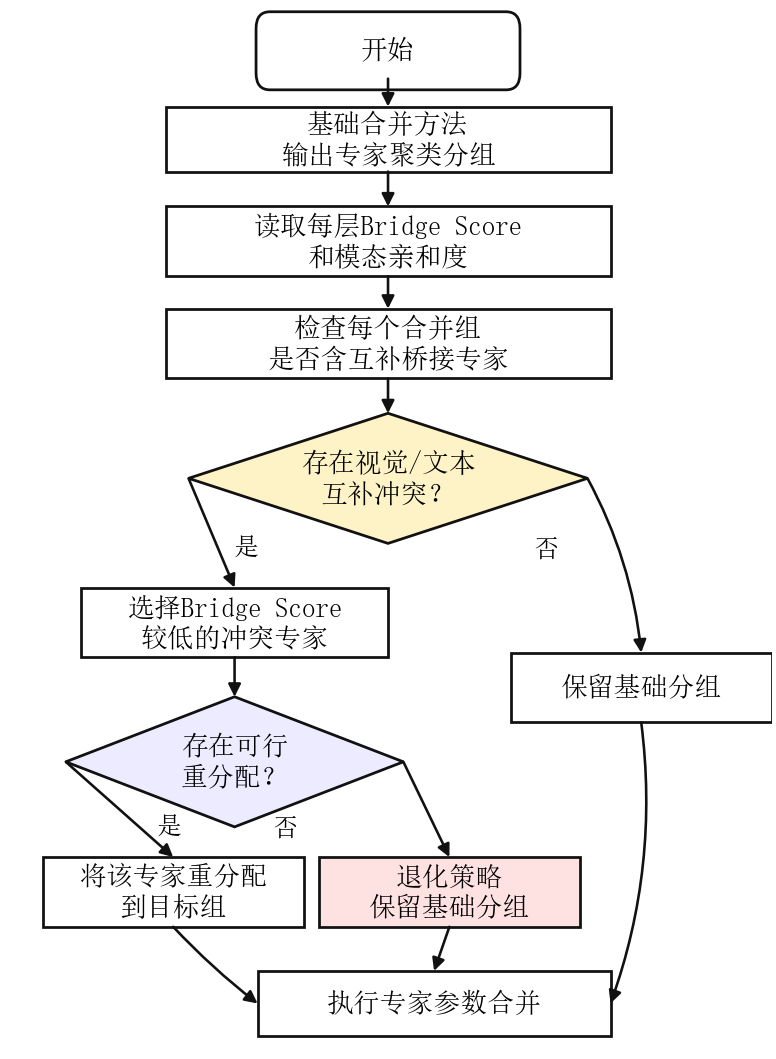
\includegraphics[width=0.70\textwidth]{images/expert_merge_flow.png}
    \caption{专家合并场景下的可容许性约束流程}
    \label{fig:merge_constraint_flow}
\end{figure}

\subsection{代码块测试}
\subsubsection{过滤器注册数据结构}
正文中出现关键数据结构或少量核心代码时，可以使用灰底斜体代码块进行展示。代码块不宜过长，通常只保留能说明设计的结构体、接口定义或关键流程。

\begin{snugshade}
\begin{cppcode}
typedef struct _DEVICE_T{
    ADD_DEVICE_FUN AddDeviceFun;        // 过滤器增加设备通知函数
    DELETE_DEVICE_FUN DeleteDeviceFun;  // 删除设备
    DELETE_DEVICE_FUN PrevDeleteDeviceFun; // 预删除设备
    DELETE_DEVICE_FUN CanDeleteDeviceFun;  // 设备是否可删除
    struct _list_t{                     // 各层过滤器连接
        void *next;                     // 该层过滤器的下层过滤器
        void *prev;                     // 该层过滤器的上层过滤器
    }list_entry;
    char MyData[1];                     // 该层过滤器私有数据
}DEVICE_T;
\end{cppcode}
\end{snugshade}

代码块之后应回到普通正文格式。本段用于检查 LaTeX 与 DOCX 转换后的段落缩进、字体和背景是否恢复正常。

\subsection{算法测试}
\algref{al:user_based_cf}给出基于用户的协同过滤推荐流程。该算法用于检查algorithm环境在LaTeX和DOCX中是否显示为标题上下双横线、输入输出无编号、步骤从1开始编号、底部横线收束的学校模板样式。

{\color{red}\bfseries 建议采用 Aurora 插件在 word 和 wps 中自动生成，相关安装使用方法请自行百度。}

\begin{algorithm}[ht]
    \caption{userBasedCollaborativeFiltering}\label{al:user_based_cf}
    \begin{algorithmic}[1]
        \Statex \textbf{输入：}\texttt{userHistory}: 所有用户的听歌历史, \texttt{userSimilarity}: 所有用户之间的相似度矩阵
        \Statex \textbf{输出：}\texttt{recommendSongsIds}: 出现次数最多的10首未听过的歌曲的ID
        \State \texttt{userSimilarities} $\leftarrow$ \texttt{userSimilarity[-1]} //计算用户与其他用户的相似度
        \State \texttt{similarUsers} $\leftarrow$ \texttt{argsort(userSimilarities)[:-6:-1]} //取相似度最高的5个用户
        \State \texttt{songsList} $\leftarrow \varnothing$
        \State \textbf{for} \texttt{user} \textbf{in} \texttt{similarUsers} \textbf{do} //保存这些相似用户听过的歌曲到集合中
        \State \hspace{1.5em}\texttt{songs} $\leftarrow$ \texttt{where(userHistory[user,:] == 1)[0]}
        \State \hspace{1.5em}\textbf{for} \texttt{s} \textbf{in} \texttt{songs} \textbf{do}
        \State \hspace{3em}\texttt{append(songsList, s)}
        \State \hspace{1.5em}\textbf{end for}
        \State \textbf{end for}
        \State \texttt{songsSet} $\leftarrow$ \texttt{set(songsList)}
        \State \texttt{recommendSongs} $\leftarrow$
        \State //计算用户未听过的歌曲，并计算评分
        \State \textbf{for} \texttt{i} \textbf{in} \texttt{range(userHistory.shape[1])} \textbf{do}
        \State \hspace{1.5em}\textbf{if} \texttt{i} \textbf{not in} \texttt{songsSet} \textbf{and} \texttt{userHistory[-1, i] == 0} \textbf{then}
        \State \hspace{3em}计算歌曲评分\texttt{score}
        \State \hspace{3em}\texttt{score} $\leftarrow$ \texttt{sum([i in songsList for user in similarUsers])}
        \State \hspace{3em}\texttt{append(recommendSongs, (i, score))}
        \State \hspace{1.5em}\textbf{end if}
        \State \textbf{end for}
        \State \texttt{sort(recommendSongs, key=lambda x: x[1], reverse=True)}
        \State \texttt{recommendSongsIds} $\leftarrow$ \texttt{[x[0] for x in recommendSongs][:10]}
        \State //返回出现次数最多的10首未听过的歌曲的ID
        \State \textbf{return} \texttt{recommendSongsIds}
    \end{algorithmic}
\end{algorithm}

\subsection{本章小结}
本章提供了数学公式、符号表、多级文字列表、图片和算法环境测试。转换后应重点检查\eqnref{eq:compression_objective}、\tabref{chart:symbols}、\figref{fig:merge_constraint_flow}和\algref{al:user_based_cf}的编号与样式。
